%%%%%%%%%%%%%%%%%%%%%%%%%%%%%%%%%%%%%%%%%%%%%%%%%%%%%%%%%%%%%%%%%%%%%%%%%%%%%%%%%%%%%%%%%%%%%
%%									section 1.	Principe Mod\`{e}le Checker Distribu\'{e}											%
%%%%%%%%%%%%%%%%%%%%%%%%%%%%%%%%%%%%%%%%%%%%%%%%%%%%%%%%%%%%%%%%%%%%%%%%%%%%%%%%%%%%%%%%%%%%%

\section{Principe Model Checking Distribu\'{e}}
 
Le model checking distribu\'{e} propos\'{e} par Bouneb Zine permet une v\'{e}rification parall\`{e}les d’une formule $\varphi$  sur les fragments de la structure de Kripke distribu\'{e}e. Du fait de la distribution, la v\'{e}rification de $\varphi$ de certain \'{e}tat \emph{S} d\'{e}pend de la v\'{e}rit\'{e} en \emph{S’} de cette formule, \emph{S’}  h\'{e}berg\'{e} dans une  machine distante $M_j$. La machine $M_i$ effectue la v\'{e}rification de $\varphi$ sur le fragment d\'{e}tenue en consid\'{e}rant la valeur logique de \emph{S’} ind\'{e}cidable  $L (\emph{S’},\varphi )=\perp$ car la formule $\varphi$ peut \^{e}tre v\'{e}rifier en \emph{S’}. Lorsque la machine $M_j$ termine le calcul est que la formule est v\'{e}rifi\'{e}e en \emph{S’}, aucune notification n'est envoy\'{e}e \`{a} la machine $M_i$, la machine $M_i$ consid\`{e}re que la formule est v\'{e}rifi\'{e}e en \emph{S’}, sinon la machine $M_j$ envoi \`{a} la machine $M_i$ la valeur logique de \emph{S’} qui est L (\emph{S’}, $\varphi$) =false. Dans ce cas, $M_i$ reprend le calcul avec la valeur envoyée pour d\'{e}terminer la v\'{e}rit\'{e}e des \'{e}tats prédécesseurs. Une fois que la terminaison est d\'{e}tect\'{e}e  la machine qui détient l’\'{e}tat initial d\'{e}duit la v\'{e}racit\'{e}e de la formule $\varphi$.

A ce principe est ajouté l'étiquetage des \'{e}tats pendant l'exécution de la de v\'{e}rification. Les \'{e}tiqu\`{e}tes associées aux \'{e}tats permettent de savoir si la valeur logique d'un état dépend de ses successeurs, ainsi que le nombre de calcul permettant de déterminer la valeur logique de l'état. A partir de ces informations il est possible  de redistribuer l'espace d’\'{e}tats afin acc\'{e}l\'{e}rer le temps du calcul de la vérification.

\begin{Exemple}
   Une structure de Kripke distribu\'{e} sur 3 machines.
   \centering
	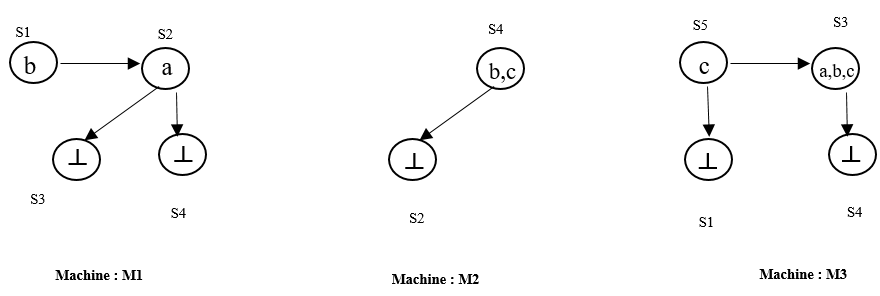
\includegraphics[height=2in]{img/skd1.png}
	
	\captionof{figure}{Structure de kripke distribu\'{e}}

\end{Exemple}

Les résultats observés durant la vérification de la formule \s{AG(a)} sont repr\'{e}sent\'{e}s dans le Tableau \ref{statistique}, les lignes repr\'{e}sentent les donn\'{e}es concernant l'\'{e}tat et les colonnes les types de donn\'{e}es construits durant le processus de v\'{e}rification. Les abr\'{e}viations utilis\'{e}es sont:
\begin{description}[,leftmargin=2cm,labelindent=1em]
	\item[Id :] L'identifiant de l’état,
	\item[T  :] Le type d’\'{e}tat (I : interne ; E : externe),
	\item[Site :] La machine distante détenant l'\'{e}tat (Externe),
	\item[RF :] La raison de la non validit\'{e} de la formule (c : che$M_i$n/ e : \'{e}tat),
	\item[i :] Le nombre de recalcul permettant de d\'{e}ter$M_i$ner la valeur logique,
	\item[VL :] La valeur logique de la formule à vérifier $(true : 1 ; false : 0 ; \perp : -1)$.
\end{description}

\begin{tableth}
	\centering
	\begin{tabular}{|*{14}{c|}}
		\hline
		\multicolumn{7}{|c|}{It\'{e}ration 1}&\multicolumn{7}{|c|}{It\'{e}ration 1}\\
		\hline
		Id&	T	&VL&	i	&Site&	M&	ME&Id&	T	&VL&	i	&RF&	M&	Site\\
		\hline
		S1	&I	&0&	1	&E	&M1	&&&&&&&&\\
		\hline
		S2	&I	&-1&	1	&M1	&&&&&&&&&\\
		\hline
		S3	&E	&-1	&1		&M1	&M3&&&&&&&&\\
		\hline
		S4	&E	&-1	&1		&M1&	M2&&&&&&&&\\
		\hline
		S2& 	E	&-1	&1	&	M2&	M1&&&&&&&&\\
		\hline
		S4	&I&	-1	&1	&	M2	&&&&&&&&&\\
		\hline
		S4	&E	&-1&	1		&M3	&M2&&&&&&&&\\
		\hline
		S5	& I&	-1 &1	&	M3	&	&S5	&I	&0	&2&	C	&M3	&&\\
		\hline
		S3&	I	&-1	&1&		M3&&&&&&&&&\\
		\hline
		S1	&E	&-1	&1	&E	&M3&	M1&	S1	&E	&0	&2	&E	&M3&	M1\\
		\hline
	\end{tabular}
	\caption{Statistique des \'{e}tats}\label{statistique}
\end{tableth}

Apr\`{e}s la premi\`{e}re it\'{e}ration l'algorithme détecte sur la machine $M_1$ que la formule n’est pas v\'{e}rifi\'{e}e sur l’\'{e}tat \s{S1}, cela permet d'envoyer une notification à la machine $M_3$ qui possède un prédécesseur direct de cet \'{e}tat. L'algorithme sur la machine $M_3$  prend en compte la modification et relance le processus de v\'{e}rification sur le fragment. La valeur logique de l’\'{e}tat \emph{S5} bascule d'indécidable à false à la deuxi\`{e}me it\'{e}ration. Apr\`{e}s cette it\'{e}ration, aucune action de modification n'est détectée, sur la machine $M_3$ l'algorithme d\'{e}duit la v\'{e}rit\'{e} de la formule.